\newpage
\section*{1 - 6}
Homeomorfizm pomiędzy
\begin{itemize}
  \item[1)] Sferą $S^n$
  \item[6)] $A = (D^p \times S^q) \cup (S^{p-1} \times D^{q+1})$ gdzie $p+q = n$
\end{itemize}
Zauważmy, że dla $z \in A$ zachodzi:
\begin{align*}
  z \in A & \implies z \in (D^p \times S^q) \lor z \in (S^{p-1} \times D^{q+1}) \\
  z \in (D^p \times S^q) & \implies \sum x_i^2 \leq 1 \land \sum y_i^2 = 1 \\
  z \in (S^{p-1} \times D^{q+1}) & \implies \sum x_i^2 = 1 \land \sum y_i^2 \leq 1 \\
  z \in A & \implies 1 \leq ||z|| \leq \sqrt{2}
\end{align*}
oraz
\begin{align*}
  z \in (D^p \times S^q) \land z \in (S^{p-1} \times D^{q+1})  & \implies z \in (S^{p-1} \times S^q)
\end{align*}
Stąd widzimy że zbiór A jest sumą dwóch rozmaitości, przecinających się w $S^{p-1} \times S^q$. Jest także prawdą, że zbiór punktów A jest izomorficzny ze zbiorem półprostych o środku w początku układu współrzędnych. Stąd istnieje projekcja punktów ze zbioru A na sferę $S^n$ przeprowadzająca punkty na przecięcia odpowiadających im półprostych ze sferą. Przekształcenie to jest bijekcją i na podobnie jak w dowodzie homeomorfizmu pomiędzy sferą a sześcianem \cite{hom-cube-sphere} jest homeomorfizmem. \\
\\
Przykładowo, dla  $(p, q) = (1, 1)$ mamy:

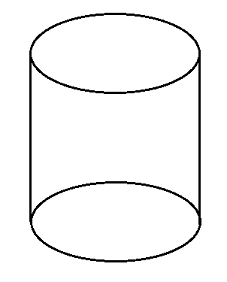
\includegraphics{cylinder.png}
